\documentclass{llncs}
\usepackage{algorithm}
\usepackage{algpseudocode}
\algtext*{EndFor}
\algtext*{EndIf}
\algtext*{EndProcedure}
%\usepackage[noend]{algorithmic}

\usepackage{authblk}
\usepackage{amsmath}
\usepackage{ulem}
\usepackage{color}
\usepackage{courier}
\usepackage{dl}
\usepackage{graphicx}
\usepackage{helvet}
\usepackage{ifsym}
\usepackage{multirow}
\usepackage{textcomp}
\usepackage{theorem}
\usepackage{times}
\usepackage{url}
\usepackage{wasysym}
\usepackage{paralist}
\usepackage{listings}
\usepackage[table]{xcolor}
\usepackage[T1]{fontenc}
\usepackage{tikz}
\def\checkmark{\tikz\fill[scale=0.4](0,.35) -- (.25,0) -- (1,.7) -- (.25,.15) -- cycle;} 

%\newdef{definition}{Definition}
%\newtheorem{theorem}{Theorem}
%\newtheorem{lemma}{Lemma}
%\newtheorem{proposition}{Proposition}
%\newdef{example}{Example}
\newcommand{\todo}[1]{\textcolor{red}{[#1]}\xspace}

\newcommand{\qn}[2]{\ensuremath{#1\mbox{:}#2}\xspace}

\newcommand{\tr}[3]{<\ensuremath{#1,#2,#3}>\xspace}

\newcommand{\B}{\ensuremath{\mathcal{B}}\xspace}

\newcommand{\V}{\ensuremath{\mathcal{V}}\xspace}

\renewcommand{\L}{\ensuremath{\mathcal{L}}\xspace}

\renewcommand{\KB}{\ensuremath{g}\xspace}

\newcommand{\itab}[1]{\hspace{0em}\rlap{#1}}
\newcommand{\tab}[1]{\hspace{.2\textwidth}\rlap{#1}}

\newlength{\hiindent}
\setlength{\hiindent}{0.5cm}
\newcommand{\hi}[1]{\hspace*{#1 \hiindent}}

\makeatletter
\let
\@copyrightspace
\relax
\makeatother


\title{How Redundant Is It? - An Empirical Analysis on Linked Datasets}

\author{Honghan Wu\inst{1} \and Boris Villazon-Terrazas\inst{2} \and Jeff Z. Pan\inst{1} \and Jose Manuel Gomez-Perez\inst{2}}
%
\authorrunning{Wu et al.}   % abbreviated author list (for running head)
%
%%%% list of authors for the TOC (use if author list has to be modified)
%\tocauthor{Panos Alexopoulos, Manolis Wallace}
%
\institute{Department of
Computing Science, University of Aberdeen, UK \and
iSOCO, Intelligent Software Components S.A., Spain}

\begin{document}


\maketitle

\begin{abstract}
Data redundancy resides in most, if not all, information systems. Linked Data is no exception. Existing approaches try to avoid data redundancies by proposing compression techniques or succinct data structures. However, data redundancies in Linked Data are useful sometimes, e.g. ontology based data access can make use of A-Box redundancies to avoid unnecessary query rewritings. Either you want to avoid it or make use of it, a good understanding about data redundancies will facilitate your task, e.g. identify the exact redundant parts which could be utilised or choose most effective techniques to compress a particular dataset. Unfortunately, little effort has been put on making the data redundancy explicit to data users. In this paper, we introduce a systematic categorisation for Linked Data redundancy, and propose an graph pattern based approach for efficient analysis.  Analysis results on representative datasets lead to a main conclusion, that is redundant-aware techniques are demanded.

\end{abstract}

\section{Introduction}
\label{sec:intro}
\textcolor{red} {@Boris}

\section{Linked Data Redundancy Categorisation}
\label{sec:gp}
Given the fact that most Linked Datasets are represented in RDF data model, in the first part of this section, we study RDF data redundancy and point out the main focuses of this paper. In addition to RDF representation, the other important characteristic of Linked Data is that it is \emph{linked}. What are the aspects of being \emph{linked} relevant to the data redundancy, and how can they be effecting it? In the second subsection we try to answer these questions.

\subsection{Redundancy in RDF Data}
\label{sec:rdf_redundancy}
From the data model level, an RDF dataset is essentially a set of triples. To share or consume an RDF dataset, e.g. for storage, transmission or query-answering, it needs to be represented in the second level, i.e. the serialisation level, where it has to be serialised as a sequence of bits. In this level, an RDF dataset usually takes the form of textual or binary files by using predefined syntaxes, e.g. RDF/XML, N-Triples or even sophisticated compression format (e.g. HDT~\cite{fernandez2013binary}). The redundancies of RDF data reside in both levels of RDF data representation, i.e. data model level and serialisation level. 

In the data model level, the size of data can be calculated by the number of triples. Hence, in this level, the data redundancy exists if less triples can be used to represent the same semantic meanings of the original data. In the serialisation level, the data is represented as a sequence of bits. Given a fix set of triples, one serialisation is said to be more redundant than the other if it uses more bits than its counterpart. 

In~\cite{wu2014ssp}, we proposed a fine-grained categorisation of RDF data redundancies. Table~\ref{tab:rdfrd} illustrates such categorisation of RDF redundancies and also puts it in the dimension of RDF representation levels. In this paper we mainly focus on the \emph{semantic redundancy} and the second type of syntactic redundancy, i.e. the \emph{inter-structural redundancy}. Both are highlighted with a grey background in Table~\ref{tab:rdfrd}. Semantic redundancy is selected because it can be generated or removed by the T-Box axioms of a dataset. Hence, it is of interest to most of the Linked Data consumption tasks like inference computation and ontology based data access. Syntactic redundancy is also important to data consumption because a concise serialisation is beneficial not only to data transmission but also to query answering tasks~\cite{fernandez2013binary}. In this category, a recent study~\cite{wu2014ssp} points out that most existing compression techniques, e.g.~\cite{fernandez2013binary}, cannot deal with the inter-structural one~\cite{wu2014ssp}. Hence, it is particularly interesting to analyse inter-structural redundancies in Linked Open Data.

\begin{table*}
\caption{RDF Data Redundancy Categorisation}
\label{tab:rdfrd}
\centering
\scriptsize
\begin{tabular}{c | c| c | c | c}
\hline
\multirow{2}{*}{Types} & \multirow{2}{*}{Semantic Redundancy} & \multicolumn{2}{c|}{Syntactic Redundancy} & \multirow{2}{*}{Symbolic Redundancy} \\
\cline{3-4}
& & Intra-structural & Inter-structural & \\
\hline
\hline
 Data Model Level  & \cellcolor[rgb]{0.9,0.9,0.9}\checkmark & - & - & -  \\
\hline
Serialisation Level & - &\checkmark &\cellcolor[rgb]{0.9,0.9,0.9} \checkmark & \checkmark   \\
\hline
\end{tabular}
\end{table*}


\begin{figure*}[t!]
\begin{center}
 \mbox{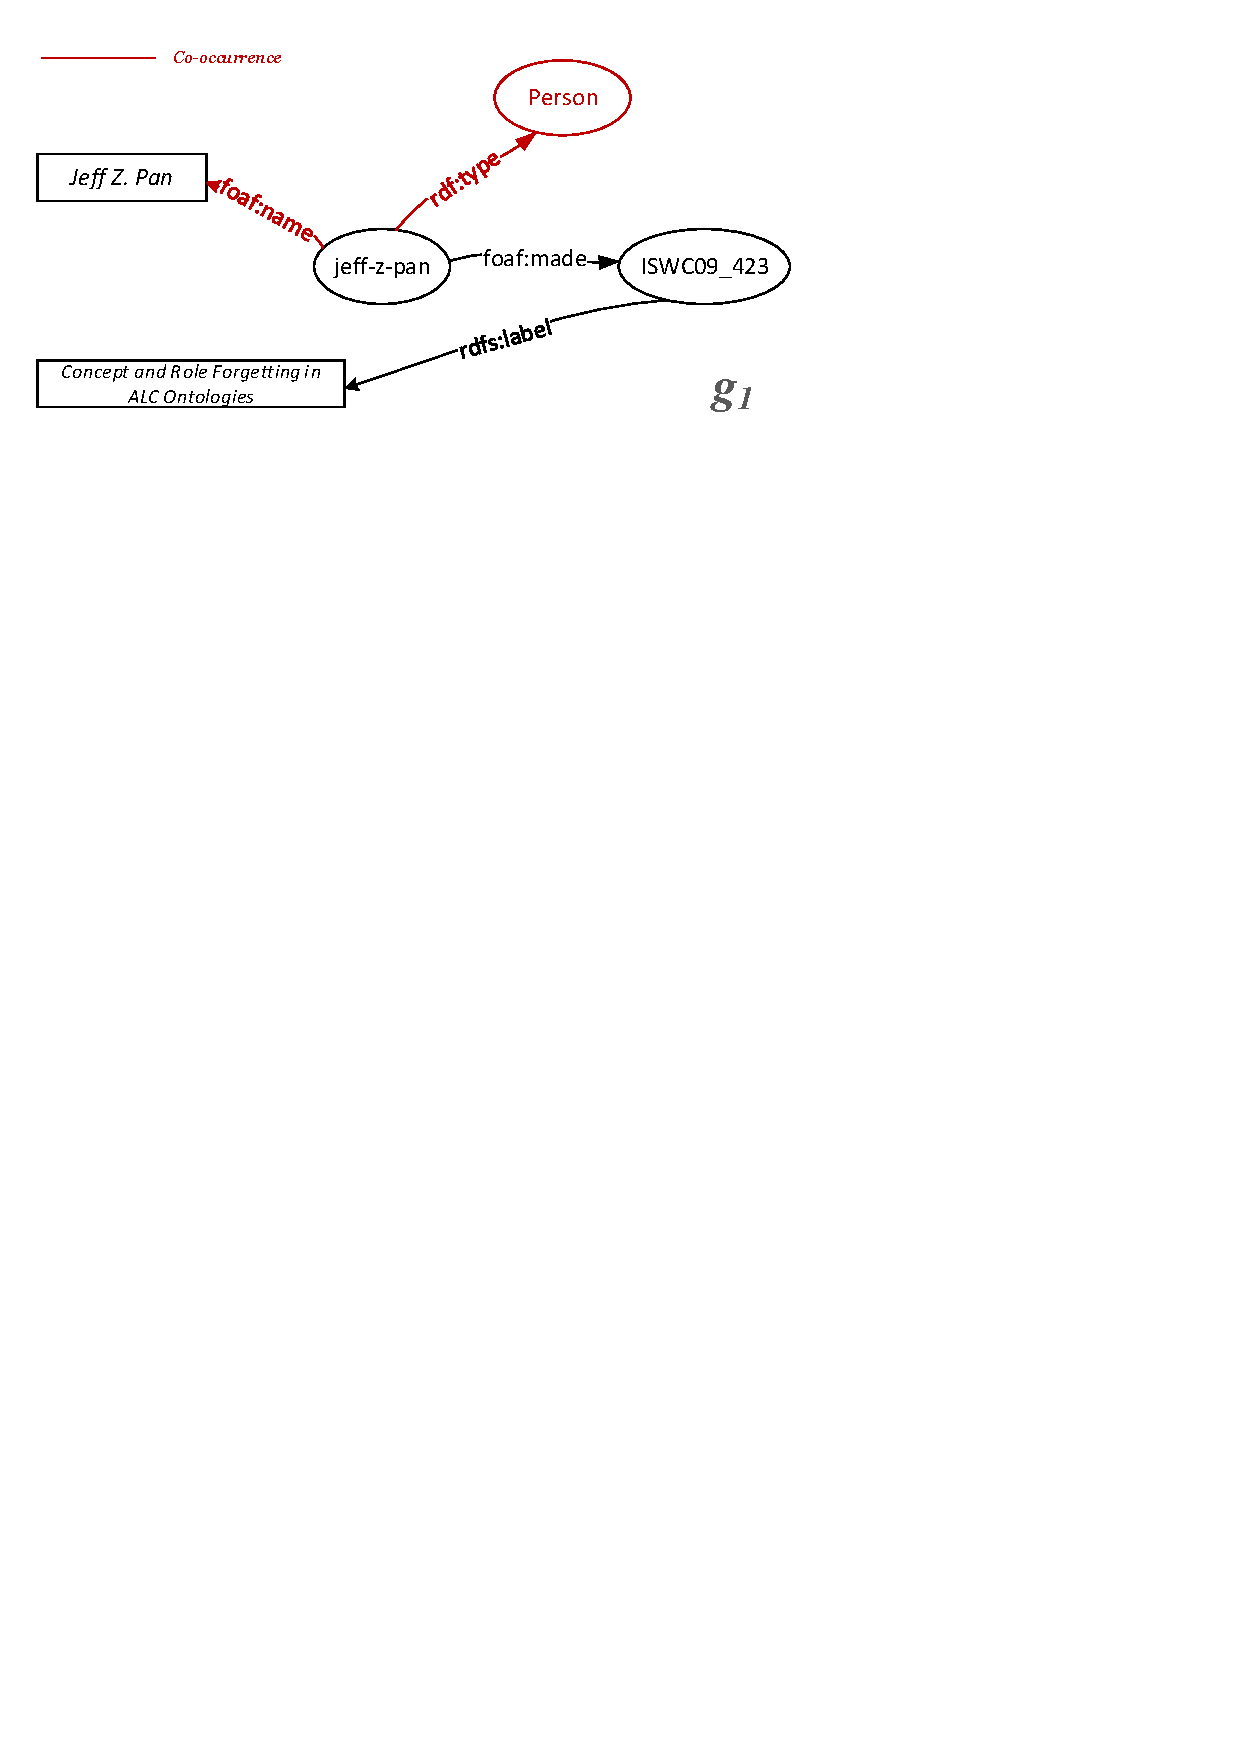
\includegraphics[scale=0.40, trim=36mm 23cm 6cm 1cm]{Figures/rd_example.pdf} }   
    \hspace{3px}
 \mbox{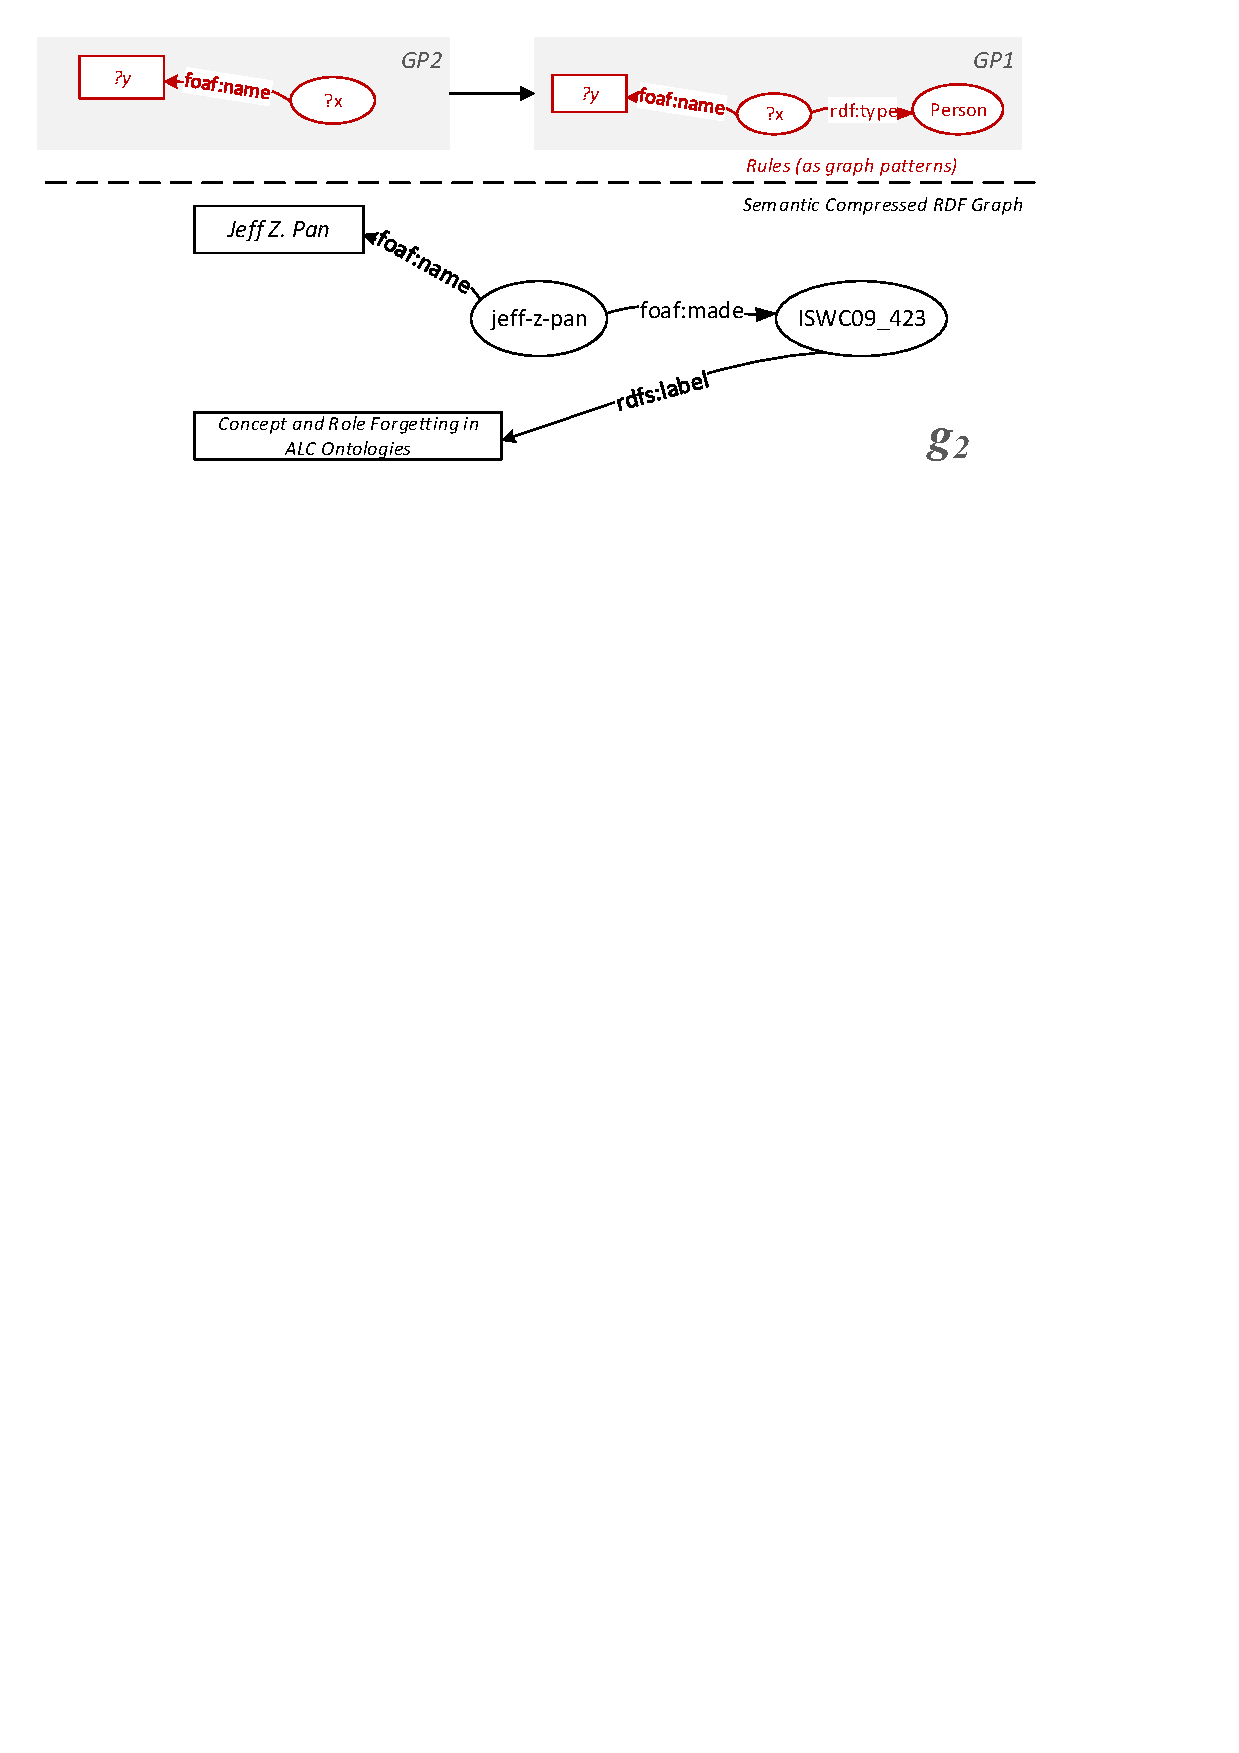
\includegraphics[scale=0.40, trim=45mm 23cm 6cm 1cm]{Figures/rd_semantic.pdf}}   
\end{center}
\caption{Original v.s. Semantically Compressed}
\label{fig:ex_orig}
\end{figure*}

{\bf Semantic Redundancy}
An RDF dataset is said to be semantically redundant if some triples can be removed without leading to any changes in its meaning. In most cases the removal of these triples requires additional rules to be added in the dataset so that it is possible to re-generate the removed triples when needed. The usual form of such rules is the T-Box, i.e., the concept level statements in an Ontology. For example, in Fig.~\ref{fig:ex_orig}, we have an RDF graph of $g_1$. In the FOAF ontology~\footnote{\url{http://xmlns.com/foaf/spec/}}, there is a rule of \tr{\qn{foaf}{name}} {\qn{rdfs}{domain}} {\qn{foaf}{Person}}. Based on the $rdfs2$ rule in the RDF specification, the type assertion in $g_1$, i.e. \tr{$jeff-z-pan$}{\qn{rdf}{type}} {\qn{foaf}{Person}}, can be removed, given the presence of \tr{$jeff-z-pan$}{\qn{foaf}{name}} {Jeff Z. Pan}.

In a more general perspective, the semantic redundancy can be identified by co-occurrences of triple patterns (cf. the red part of $g_1$ in Fig.~\ref{fig:ex_orig}). Hence, it is not necessary to restrain the ability of semantic redundancy identification by the limitation of T-Box rules in representing triple pattern co-occurrences. In this regard, Joshi et al.~\cite{joshi2013logical}  applied association rule mining approach to identify the co-occurrences in terms of association rules. In this paper, we apply a graph pattern based rule system to represent the semantic redundancies. For example, in Fig.~\ref{fig:ex_orig}, $g_2$ has less triples than $g_1$ but the two are semantically equivalent. The redundancy in $g_1$ is represented by the graph pattern rule in the upper part of $g_2$. Obviously, graph pattern based rules can represent more complex triple co-occurrences than T-Box rules.

{\bf Inter-structure Syntactic Redundancy}
As shown in Table~\ref{tab:rdfrd}, the other two types of redundancies, i.e. syntactic and symbolic ones, both resides in the serialisation level. Their volume can be evaluated using the number of bits used in the serialisation. To separate the two, we can use a simple formula $|F| = n \times r$, where $F$ is the serialisation file, $n$ is the number of resource occurrences and $r$ is the average bits needed to represent a resource. The syntactic redundancies reside in the component of $n$, while the symbolic ones are in $r$.

Most existing serialisation approaches apply syntaxes to reduce $n$. The idea is to group triples by subjects or objects so that the multiple occurrences of the same resource only need to be serialised once. For example, the RDF/XML serialisation standard provides abbreviation and striping syntaxes. However, such syntaxes only work on concrete graph structures. Similar graph structures (i.e. graph patterns)  which repeatedly occur in the data are not taken into account. In the following example, the graph pattern $GP$ has two instances of $Inst_1$ and $Inst_2$. The structure of $GP$ appears twice in both instances. This means that each of the two predicate resources of $GP$, i.e. \qn{foaf}{name} and \qn{foaf}{made}, has two occurrences in its instances, which is avoidable when $GP$ structure (stored wherever) is referred instead of duplicated in both instances.

\scriptsize
\begin{align}
GP: &\tr{?U} {\qn{foaf}{name}} {?Y},  \tr {?U}{\qn{foaf}{made}} {?Z}\nonumber\\ 
Inst_1: &\tr{\text{\it jeff-z-pan}} {\qn{foaf}{name}} {\text{Jeff Z. Pan}},  \tr {?U}{\qn{foaf}{made}} {ISWC09\_423}\nonumber\\ 
Inst_2: &\tr{jose} {\qn{foaf}{name}} {\text{Jose Manuel Gomez Perez}},  \tr {?U}{\qn{foaf}{made}} {ISWC13\_1xx}\nonumber
\end{align}
\normalsize

We use the term of \emph{intra-structural redundancy}  to denote the unnecessary resource occurrences in concrete graph structure, while  the term of \emph{inter-structural redundancy} is used for the unnecessary resource occurrences of graph patterns in its instances. Most of existing serialisation approaches do not provide facilities to identify graph patterns. Hence, they leave the inter-structural redundancy untouched.

\subsection{Redundancy in Linked Data}
One of the most important characteristics of Linked Data is its \emph{linking} capability, which is to create connections from one information source to the other. The connection can be created in the concept level, where individuals of one dataset are described using concepts from another dataset or vocabulary. We denote this type of connections as \emph{T-Box Reuse}. The second type of connections is the linkage in individual level, where individuals in one dataset are specified to be the same as their counterparts in the other, e.g. by using \qn{owl}{sameAs} assertions. This type of connections is called as \emph{A-Box Linkage} in this paper. Both types of connections have implications in changing the semantics of the original dataset. These implications might change the redundancies of the dataset in question. In rest part of this subsection, we briefly discuss the possible changes on data redundancies caused by \emph{T-Box Reuse}, and leave the \emph{A-Box Linkage} for future work.

\subsubsection{T-Box Reuse}
Essentially, T-Box Reuse will bring new rules to the original dataset. These rules are a subset of the materialised axioms of the reused T-Box, which are applicable to the individual. These new rules can infer a set of new triples~\footnote{Some triples inferred by new rules might be inferred by the dataset\rq{}s own T-Box as well. To make discussion easier, we use the term {\it new triples} to denote those triples which can NOT be inferred by the dataset\rq{}s own T-Box but the new rules.} to the reusing RDF dataset. 

\begin{figure}
\begin{center}
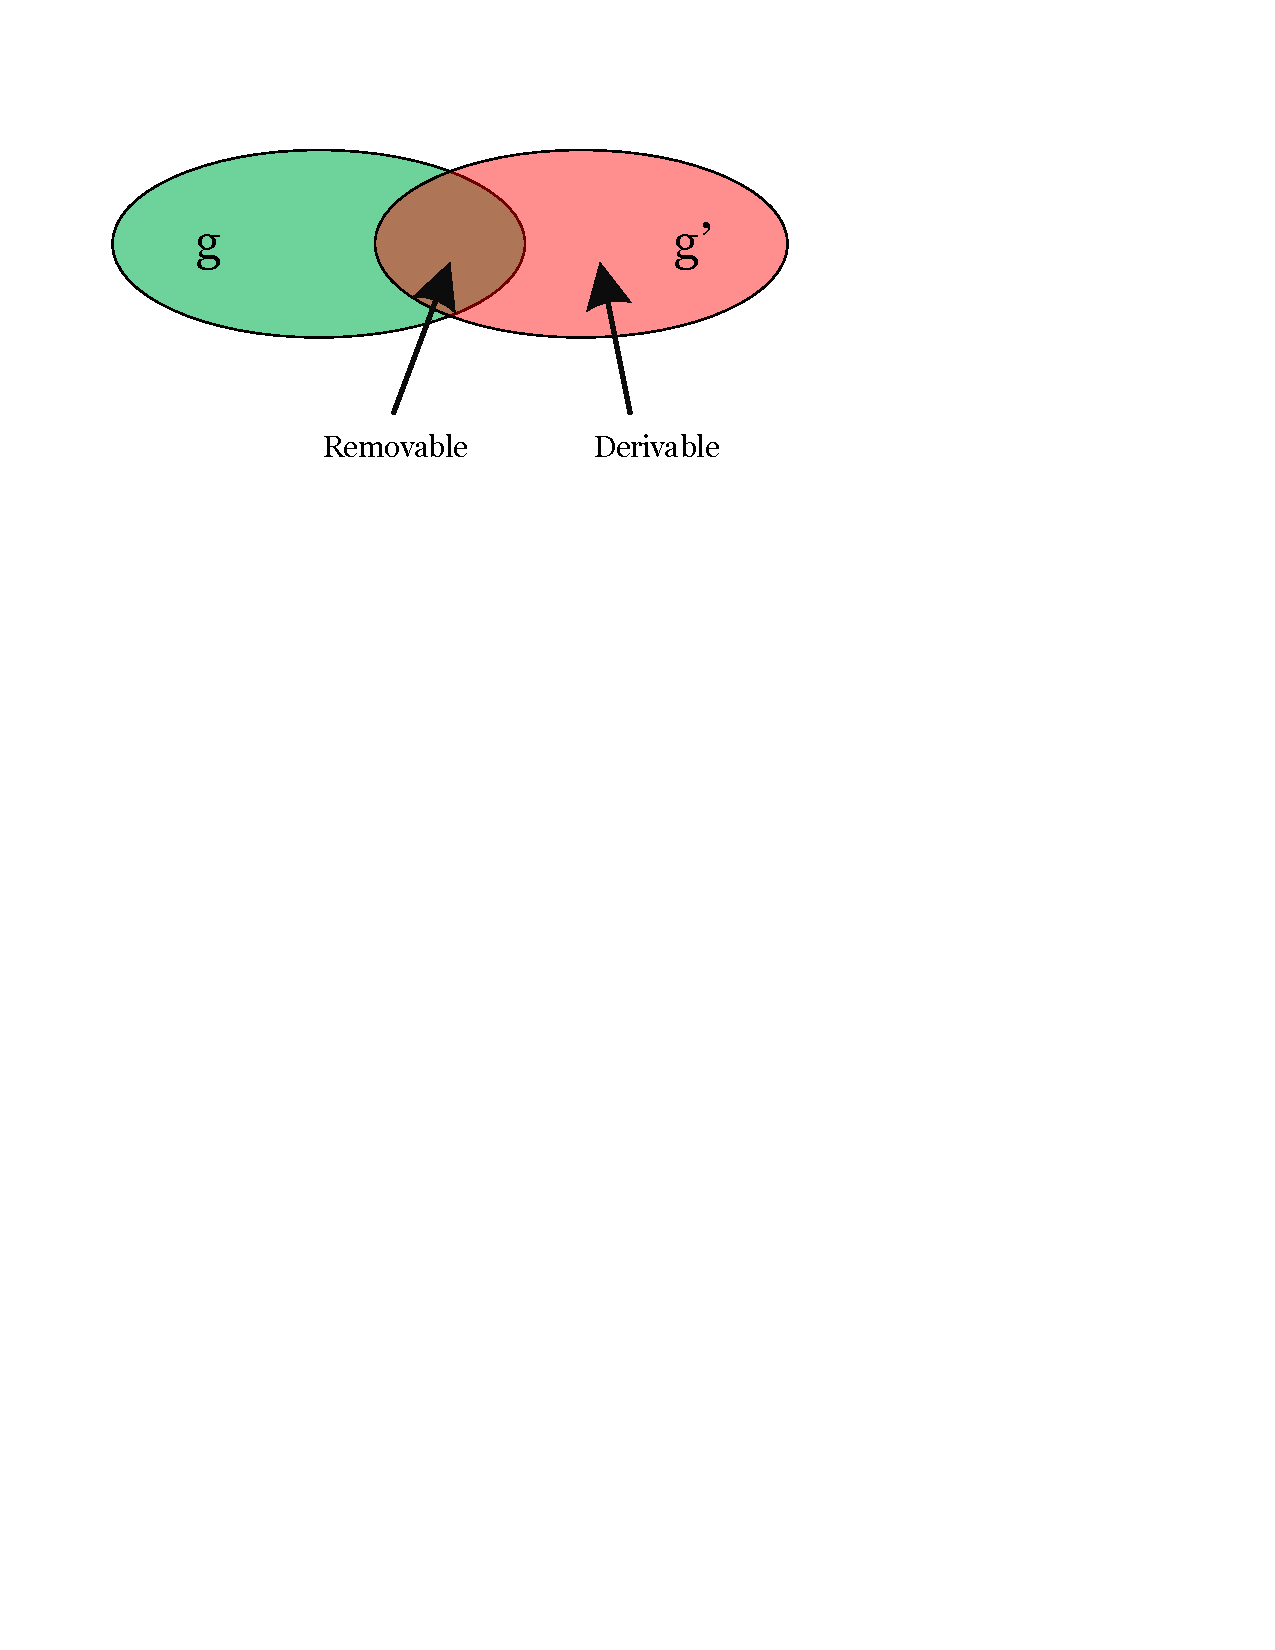
\includegraphics[scale=0.40, trim=36mm 22cm 9cm 3.5cm]{Figures/tbox_reuse.pdf}  
\end{center}
\caption{Data Redundancies affected by T-Box Reuse}
\label{fig:tbox_reuse}
\end{figure}



 Fig.~\ref{fig:tbox_reuse} illustrates a typical case of such inference results. In Fig.~\ref{fig:tbox_reuse}, the original RDF dataset, labelled as $g$, is denoted by the green oval, and the new set of inferred triples is denoted by the pink oval with a label of $g\rq{}$. Depending on whether they are in the overlap with existing triples, new triples can be divided into two parts. The two parts will lead to two different consequences to the redundancies of the original data. The overlap part, labelled \emph{$removable$} in Fig.~\ref{fig:tbox_reuse}, contains those triples in $g$, which can be inferred by new rules as well. This means that they are turned to be semantically redundant by the reused T-Box. As a consequence, the dataset turns to have more redundancies. On the contrary, the other part ($g\rq{} \setminus removable$), labelled as \emph{$derivable$} in Fig.~\ref{fig:tbox_reuse}, will decrease the data redundancy by means of increasing data compression ratio. According the definition of data compression ratio~\footnote{\url{http://en.wikipedia.org/wiki/Data_compression_ratio}}, it can be calculated by $\frac{|g| + |derivable|}{|g|}$, in which the bigger $|derivable|$ component becomes, the larger the compression ratio will be. 
 
 To sum up, $removable$ and $derivable$ affect the data redundancies in opposite ways. Analyses on them will reveal the effects on data redundancy of concept-level connections between Linked Data.  

%{\bf A-Box Linkage}
%Individual level linkages by \qn{owl}{sameAs} assertions are among the most advocated best practices in the Linked Data community. Data publishers are encouraged to provide such linkages to break the information silos. However, its semantic implications will lead to substantial inference computations across different datasets, some of which might be unexpectedly expensive. In~\cite{halpin2010owl}, Halpin et al. pointed out that {\it quick-and-dirty use of \qn{owl}{sameAs} will almost always lead to OWL Full}. The other issue is that transitive closures of \qn{owl}{sameAs} in the Web scale can easily get too large to be manageable.
%
%Despite the practical issues, we briefly discuss how the semantic implications of \qn{owl}{sameAs} links might lead to the changes in data redundancies. As supporting efficient query answering is the basis of many Linked Data consumption tasks, our discussion in this paper is based on OWL2 QL profile~\cite{calvanese2007tractable}. When an individual $i$ in dataset $D$ is asserted to be {\it sameAs} another individual $i_1$ in $D_{i_1}$, all \emph{materialised assertions} of $i_1$ in $D_{i_1}$, denoted as $A(i_1)$, are immediately true to $D$. Hence, the data of D will be $g_D \cup A(i_1)$, where $g_D$ is the original RDF graph of D. Considering OWL2 QL semantics, it is reasonable that only type assertions of $i_1$ in $D_{i_1}$ are included in $A(i_1)$ directly. Regarding other triples of $i_1$ in $D_{i_1}$, they will be simplified as existential assertions to be added.
%
%Similar to T-Box Reuse case, the adding of new data has two consequences to the data redundancy of D. The first one is some triples turned to be redundant, while they were not originally. We also use the term \emph{\it removable} to denote these triples. Let $M$ be an A-Box materialisation function. The \emph{\it removable} can be calculated by ${\it removable}=g_D \cap \big( M(g_D \cup A(i_1)) \setminus M(g_D) \big)$. The second consequence is that $g_D$\rq{}s data compression ratio can be increased, which means less redundancy. This is caused by new triples which are not in the original data and turn to be derivable after adding $A(i_1)$, while they could not be derived before that. The term \emph{\it derivable} is used to denote such triples, which can be calculated by $derivable=\big( M(g_D \cup A(i_1)) \setminus M(g_D) \big) \setminus g_D$.


\section{Two Dimension Analysis}
\label{sec:method}

According to above discussions, the redundancies in Linked Data can be analysed from two dimensions (cf. Fig.~\ref{fig:twod}). The first dimension is that of the RDF data redundancy, where the focus is to reveal different categories of redundancies from data model level to serialisation level. The second dimension is from the \emph{linked} semantic point of view, where the focus is to analyse the data redundancy based on different types of semantics. The {\it A-Box } semantics is to analyse the data redundancy only from data level without any T-Box axioms. The other three types are considering both data and T-Box information. The {\it No Linkage} semantics is to do the analysis based on the dataset\rq{}s main T-Box. The main T-Box is the one most used for describing individuals in the data, which is either defined by the data provider or reused from other sources. In our analysis, we manually identify such main T-Box for each dataset. It is not necessary that every dataset has a main T-Box. In such cases, this analysis is not applicable. The {\it T-Box Reuse} semantics is the type of analysis focusing on redundancy changes caused by concept level connections, i.e. reusing T-Box, while the {\it A-Box Linkage} is to reveal the changes of data redundancies caused by the individual level connections.

\begin{figure}
\begin{center}
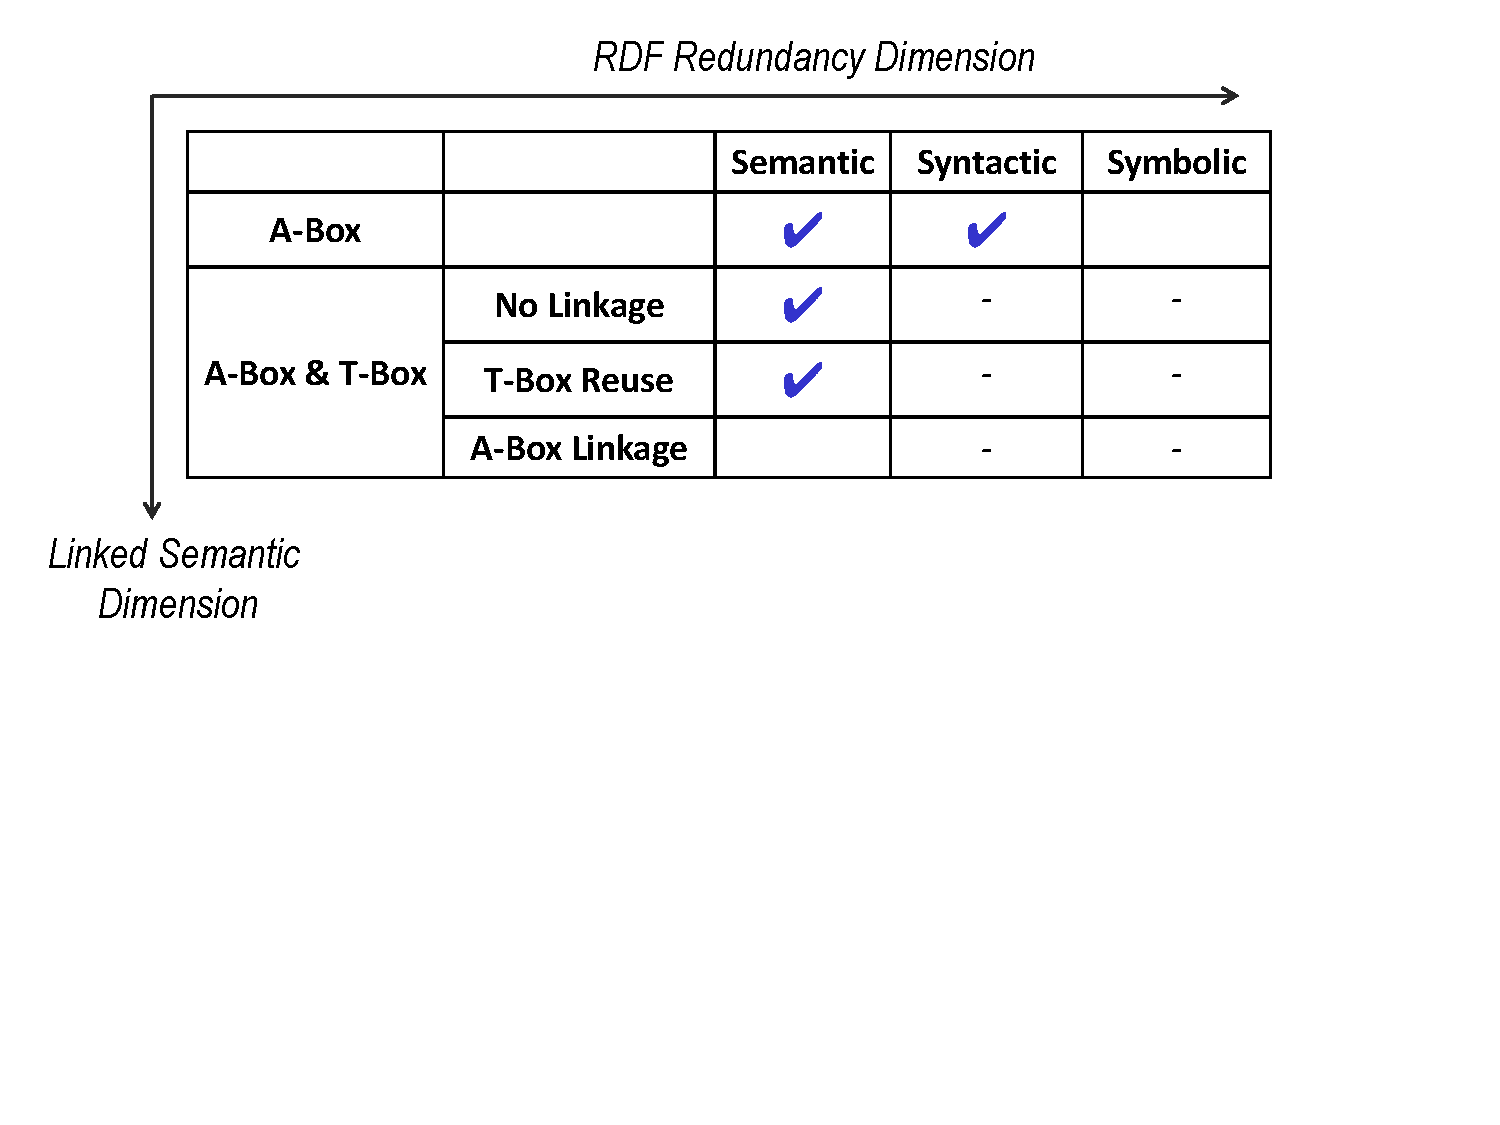
\includegraphics[scale=0.35, trim=6cm 10cm 6cm 2cm]{Figures/two_dimension.pdf}  
\end{center}
\caption{Two Dimension Analysis on Linked Data Redundancy}
\label{fig:twod}
\end{figure}

In the matrix of Fig.~\ref{fig:twod}, there are total 6 valid types of analyses. In this paper, we focus on four of them, which are marked with ticks in the figure. For {\it A-Box} semantics, we propose a graph pattern based approach to reveal the semantic and syntactic (inter-structure only) redundancies. Based on the graph pattern approach, we propose a virtual materialisation approach to analyse data redundancies in {\it No Linkage} and {\it T-Box Reuse} semantics. The other two types of analyses are left for future work.


\subsection{Graph Pattern Based Analysis Method}
As discussed in section~\ref{sec:rdf_redundancy}, we focus on semantic redundancy and the inter-structural syntactic redundancy, both of which will be benefited from the ability to identify frequent graph patterns. For semantic redundancy, identified graph patterns can be used to identify possible rules for removing redundant triples. Combined with the knowledge of instance numbers of these graph patterns, these rules can be used to calculate the volume of semantic redundancy as number of removable triples. Similarly, for inter-structural redundancy, the structure of graph patterns and their instances numbers can give us a way to calculate the volume of syntactic redundancy in the data. In this subsection, we describe an entity description pattern based approach for redundancy analysis.

In an RDF graph, we call its non-literal nodes as entities. For an entity $e$ in an RDF graph $G$, we can get a data block for it by extracting triples in $G$ each of which has $e$ as its subject or object. We call such kind of data blocks as Entity Description Blocks (EDBs for short). 

For an EDB, it can be summarised by a notion of entity description pattern which is defined in Definition~\ref{def:edp}. \emph{EDP}, the short name for entity description pattern, is the building block of our analysis approach. 

\begin{definition}
\label{def:edp} 
(Entity Description Pattern) Given an entity description block $B_e$, its description pattern is a tuple $P_e=(C_e,A_e,R_e,V_e)$, where
\begin{itemize}
\item $C_e=\{c_i |<e, rdf:type,c_i> \in G\}$   is called as the class component; 
\item $A_e=\{p_i |<e,p_i,l_i> \in G \text{ and $l_i$  is a literal}\}$  is called as the attribute component;
\item $R_e=\{r_i |<e,r_i,o_i> \in G \text{ and $o_i$  is a URI resource or blank node}\}$  is called as the relation component;
\item $V_e=\{v_i |<s_i,v_i,e> \in G\}$ is called as the inverse relation component.
\end{itemize}
\end{definition}

Taking the RDF graph $g_1$ in Fig.~\ref{fig:ex_orig} for example, the EDP of entity {\it jeff-z-pan} is $\big( \{\qn{foaf}{Person}\}, \{\qn{foaf}{name}\}, \{\qn{foaf}{made}\}, \emptyset \big)$, and the one of {\it ISWC09\_423} is $\big( \emptyset, \{\qn{rdfs}{label}\}, \emptyset , \{\qn{foaf}{made}\}\big)$. 

\vspace{1ex}

By generating EDPs for all entities in an RDF graph $G$, we can get a EDP representation of $G$, which is a set of EDPs. As we will show in later section, the number of EDPs in an RDF dataset is usually much less than the number of entities. This is because many entities are sharing same EDP. The more entities are sharing one EDP; the more frequent its structure is duplicated. Such duplications are the source of data redundancies, which we break down to semantic redundancy and syntactic redundancy.

\vspace{2 mm}

\noindent {\bf Semantic Redundancy Identified By EDP} In the definition of EDP, the class component $C_e$ is a set of constant class names. Hence, it is straightforward to generate a graph pattern based substitution rule for removing these type assertions from the original data. In particular, the substitution rule is defined as $(\emptyset, A_e, R_e, V_e) \rightarrow (C_e,A_e,R_e,V_e)$. Let $f_{P_e}$ be the instance number of $P_e$, the number of triples can be removed by the rule is $|C_e| \times f_{P_e}$. In {\it jeff-z-pan}\rq{}s example, the rule will be $(\emptyset, \{\qn{foaf}{name}\}, \{\qn{foaf}{made}\}, \emptyset) \rightarrow ( \{\qn{foaf}{Person}\}, \{\qn{foaf}{name}\}, \{\qn{foaf}{made}\}, \emptyset)$. In this particular case, this rule is equivalent to the rule of \tr{\qn{foaf}{name}} {\qn{rdfs}{domain}} {\qn{foaf}{Person}} from $FOAF$ vocabulary. 

\vspace{2 mm}

\noindent {\bf Inter-structural Syntactic Redundancy Identified By EDP} The inter-structural redundancy denotes the unnecessary structure recurrences in EDP\rq{}s instances, i.e. EDBs. Given an EDP $P_e$, it is straightforward to calculate its recurrences as $(|A_e| + |R_e| + |V_e|) \times f_{P_e}$,  the unit of which is resource occurrence.

\vspace{2 mm}

\noindent {\bf Virtual A-Box Materialisation on EDP} When considering T-Box of an RDF dataset, the data redundancy might be changed due to the above-mentioned $removable$ and $derivable$ triple sets. To compute the two triple sets, inferences need to be performed on A-Boxes, which might be too expensive for large scale data analyses. For redundancy analysis purpose, we only need to know the size of $removable$ and $derivable$ sets instead of getting the exact triples. Inspired by this observation, we propose a virtual materialisation approach based on EDP to compute the triple sizes for the two triple sets. 

As supporting efficient query answering is the basis of many Linked Data consumption tasks, our discussion in this paper is based on OWL2 QL profile~\cite{calvanese2007tractable}. Given an EDP $P_e$, according OWL2 QL profile, it can be proved that the four components of $P_e$ are sufficient for inference computation on EDP. When applying inference rules defined in~\cite{calvanese2007tractable} on an EDP, we use a new EDP: $P_e^M=(C_e^M, A_e^M, R_e^M, V_e^M)$ to store all the inference results. After the inference, the number of {\it derivable} triples can be calculated as follows. 

\begin{equation}\label{eq:derivable}
 |derivable|=f_{P_e} \times \sum_{c \in N}f(c),
\end{equation}
\indent {\it where $N=( C_e^M \setminus C_e ) \cup ( A_e^M \setminus A_e ) \cup ( R_e^M \setminus R_e ) \cup ( V_e^M \setminus V_e )$ and $f$ is an auxiliary dictionary  which stores the instantiated times of each concept in $P_e \cup P_e^M$.}

\vspace{1ex}

The number of {\it removable}  triples can be calculated as follows.
\begin{equation}\label{eq:removable}
 |removable|=f_{P_e} \times \sum_{c \in E}f(c),
\end{equation}
\indent {\it where $E=( C_e^M \cap C_e ) \cup ( A_e^M \cap A_e ) \cup ( R_e^M \cap R_e ) \cup ( V_e^M \cap V_e )$.}

\section{Related Work}
\label{sec:related}
RDF compression techniques have been proposed to eliminate data redundancies. Such as RDF serialisations techniques, i.e. HDT serialisation~\cite{fernandez2013binary}, lean graphs~\cite{iannone2005optimizing} and K2-triples~\cite{alvarez2011compressed} can be used to reduce file size. Another approach is based on logical compression, such as the rule-based RDF compression~\cite{joshi2013logical}, which can be used to substantially reduce the number of triples in an RDF document. Inspired by the HDT approach, Cur{\'e} et al. proposed WaterFowl ~\cite{cure2014waterfowl} as a succinct data structure for RDF data. The OWL sameAs network was studied by Ding et al.~\cite{ding2010sameas}. The implication of sameAs links was raised but not studied. Halpin et al.~\cite{halpin2010owl} also proposed a way to analyse identity in linked data based on sameAs links. As we mentioned, none of existing work has made the data redundancies explicit and available to stakeholders of Linked Data, which is the main focus of this paper.

\section{Redundancy Analysis Results on Linked Datasets}
\label{sec:result}
%\subsection{The Metrics}
%\begin{table}
%\caption{Linked Data Redundancy Analysis Metrics}
%\label{tab:metrics}
%\centering 
%\resizebox{\textwidth}{!}{
%\begin{tabular}{c | c| p{2.2cm} | p{2.2cm} | p{2.2cm}}
%\hline
%\multicolumn{2}{c|}{ } & {\bf General Info} & {\bf Semantic@90\%} & {\bf Syntactic@90\%}\\
%\hline
%\hline
%\multicolumn{2}{c|}{A-Box} 
%%general info
%& {\it \# Triples \newline \# EDP \newline \# EDP@90\%   }
%%semantic of A-Box only
%& {\it \# RTriple \newline $RRatio_{sem}$ \newline \#GP Rules}
%%syntactic
%&  \# $RRes$ \newline $RRatio_{syn}$
%\\
%\hline
%\multirow{2}{*}{A-Box \& T-Box } & No Linkage & \multirow{2}{*}{ - }  
%%Semantic of No-Linkage
%& {\it \# derivable \newline \# removable  }
%&  \multirow{2}{*}{ - }  \\
%\cline{2-2}
%\cline{4-4}
%&  T-Box Reuse & 
%%Semantic of T-Box Reuse
%& {\it \# derivable \newline \# removable \newline  \#DTerm \newline \#RAxioms}
%&  \\
%\hline
%\end{tabular}}
%\end{table}


\subsection{Datasets}
The datasets selected for analysis are identified from Linked Open Data cloud~\footnote{\url{http://lod-cloud.net/}}. There is a coloured version which categorises the datasets in different domains. We selected 5 datasets from the Linked Open Data Cloud, which cover 5 out 6 domains listed in the coloured version. The general information about datasets is listed in Table~\ref{tab:data}.

\begin{table*}
\caption{General Information of Selected Datasets}
\label{tab:data}
\scriptsize
\centering
\begin{tabular}{p{2.2cm} | p{2.2cm}  | r| r | r }
\hline
Dataset &Domain  & $\#$Triples  & $\# EDP$ & $\# EDP@90\%$    \\
\hline
\hline
 LinkedMDB  & Media & 6,148,121 & 10,316  &   26 \\
 \hline
 LOV &User-generated content & 54,630 &492	 &  15   \\
\hline
DBLP &Publication &  94,450,169 & 438	 & 6 \\
\hline
Ordnance Survey \newline (50K Gazetteer) &Geographic \newline \& Government &2,368,655	 & 6 & 1 \\
\hline
Ordnance Survey \newline (Code-Point) & Geographic \newline  \& Government & 33,750,456 & 19 & 2\\
\hline
\end{tabular}
\end{table*}

In addition to trying to have a diverse domain coverage in dataset selection, we tried to select datasets with different sizes (cf. the $\#Triples$ column). We also selected two different datasets from one particular dataset (the Ordnance Survey), which are quite different in topics and size. The main purpose is to have our sample as representative as possible, while keeping the number of datasets manageable.

One strategy we apply in our analyses it to focus on data instances of most popular EDPs instead of working on all data. The idea is to maintain an efficient analysis while capturing the most part of the data. The threshold chosen is 90\%, which means that we analysis 90\% of the data. 

In the table, there are other metrics related to EDP. $\#EDP$ is the total number of EDPs identified in the dataset, which is a quantitative measurement about the variety of how entities are described. $\# EDP@90\% is $ means the minimal number of top popular EDPs the sum of whose instance numbers is not less than 90\% of the total number of entities in the dataset. From Table~\ref{tab:data}, although the total number of EDPs are large in some cases, e.g. LinkedMDB has more than 10 thousand EDPs, the major part of the data (90\%) resides in a very small number of EDPs in all cases. The more popular one EDP is; the more redundancy there will be. Hence, having a small number of very popular EDPs indicates a large volume of data redundancies.
\subsection{The results}
\noindent {\bf A-Box only results}
Table~\ref{tab:ret_abox} gives the analysis results by only considering A-Box level information. Both syntactic and semantic redundancies are analysed by EDP based approach. In the table, $\# RRes$ is the redundant resource occurrences of inter-structural redundancies; $RRatio_{syn}$ is the syntactic redundancy ratio, i.e. $\frac{\# RRes /3}{\# Triples}$; $\# RTriple$ is the redundant triples (i.e. semantic redundancy); $RRatio_{sem}$ is the semantic redundancy ratio, i.e. $\frac{\# RTriple}{\# Triples}$; and $\# GP Rules$ is the number of graph pattern substitution rules needed to remove semantic redundant triples.

As for \emph{syntactic redundancies}, in all datasets, they are considerably large. The redundant ratio is more than 20\% in all cases except DBLP where the ratio is still near 6.5\%. The biggest ratio was obtained from {\it 50K Gazetteer}, which is more than 32\%. Furthermore, it is notable that we only consider inter-structural redundancy and the ratio is calculated from redundancies in 90\%  data over the whole data. This means that the overall syntactic redundancy ratio should be even more.

\begin{table*}
\caption{A-Box Only: Semantic Redundancy and Syntactic Redundancy}
\label{tab:ret_abox}
\centering
\scriptsize
\begin{tabular}{p{2.2cm} | r | r|| r | r | r}
\hline
\multirow{2}{*}{Dataset} & \multicolumn{2}{c||}{Syntactic Redundancy} & \multicolumn{3}{c}{Semantic Redundancy} \\
\cline{2-3}
\cline{3-6}
 & $\#RRes$ & $RRatio_{syn}$ & $\#RTriple$ & $RRatio_{sem}$ & $\#GP Rules$   \\
\hline
\hline
 LinkedMDB  & 4,475,952	 & 24.27\% & 610,463  &   9.93\% & 21 \\
 \hline
 LOV & 36,718	 & 22.40\%	 &8,845 &  16.19\% & 8	   \\
\hline
DBLP &18,283,964	 &  6.45\%	 & 2,901,347 &  3.07\%	 & 3 \\
\hline
Ordnance Survey \newline (50K Gazetteer) &2,331,720 &32.81\%	 & 259,080 & 10.94\% & 1 \\
\hline
Ordnance Survey \newline (Code-Point) & 27,455,294 & 27.12\% & 1,595,931 & 4.73\% & 3\\
\hline
\end{tabular}
\end{table*}

The right part of Table~\ref{tab:ret_abox} shows that the EDP approach can identify substantial semantic redundancies as well. More than 3\% of triples are redundant in all analysed datasets. The most semantically redundant one is {\it LOV} dataset, which has more than 16\% redundant triples. The $\# GP Rules$ column shows an interesting phenomenon, i.e. these semantic redundancies can be removed by very small number of rules. The most efficient rule set comes from {\it 50K Gazetteer}, where one single rule can remove more than 10\% triples.

\noindent{\bf Linked Semantics}
Table~\ref{tab:ret_tbox} shows the data redundancies under different explicit semantics. Two types of semantics of {\it No Linkage} and {\it A-Box Reuse} are analysed. $\# DTerm$ is the number of terms from reused T-Box, which are directly used by current dataset; and $\# RAxioms$ is the number of  axioms from (materialised) reused T-Box, which are used for virtual materialisation on EDPs in the dataset.

{\it No Linkage} analyses are done by considering the datasets\rq{} main T-Boxes. As shown in left part of Table~\ref{tab:ret_tbox}, {\it LinkedMDB} and {\it LOV} do not have a main T-Box. They are using concepts defined in their own name spaces but without specifications about the semantics of these concepts. Such situations are very common in Linked Data Cloud. For {\it DBLP} dataset, we identified its main T-Box as SWRC ontology~\footnote{\url{http://ontoware.org/swrc/}}. Considering this T-Box, there will be 1.6 million triples can be further derived but no triples in the dataset are removable. This means that the current data is semantically less redundant when T-Box axioms are taken into account. The case of {\it 50K Gazetteer} is similar, where main ontology of the dataset is officially published~\footnote{\url{http://data.ordnancesurvey.co.uk/datasets/os-linked-data}}. However, it is worth mentioning that the $derivable$ triples of {\it 50K Gazetteer} are even more than its original triples. In {\it Code-Point}\rq{}s case, the T-Box can help remove around 1.6 million triples. This means that these triples turn to be redundant.

\begin{table*}
\caption{Linked Semantics: Data Redundancies Considering (Linked) T-Box Axioms}
\label{tab:ret_tbox}
\centering
\scriptsize
\begin{tabular}{p{2.2cm} | r | r|| r | r | r | r}
\hline
\multirow{2}{*}{Dataset} & \multicolumn{2}{c||}{No Linkage} & \multicolumn{4}{c}{T-Box Reuse} \\
\cline{2-3}
\cline{3-7}
 & $derivable$  & $removable$ & $derivable$  & $removable$& $\#DTerms$ & $\#RAxioms$   \\
\hline
\hline
 LinkedMDB  &  -	 & -   & 1,652,385   &   0  & 2 & 6\\
 \hline
 LOV & -	 & -	 &2,197 &  0 & 2 & 11	   \\
\hline
DBLP &1,669,644		 & 0	 & 42,851,260 &  1,231,703	 & 2 & 10 \\
\hline
Ordnance Survey \newline (50K Gazetteer) &4,361,100 &0	 & - &- & - & - \\
\hline
Ordnance Survey \newline (Code-Point) & 36,706,413 & 1,595,931&- &- & - & -\\
\hline
\end{tabular}
\end{table*}

The right part of Table~\ref{tab:ret_tbox} gives the analysis result of considering reused T-Box axioms. 3 out of 5 datasets are reusing one popular T-Box, i.e. FOAF ontology. In {\it LOV} dataset, about 4\% new triples can be inferred by the reusing FOAF ontology. In other two cases, {\it LinkedMDB} and {\it DBLP}, a surprisingly large number of triples can be derived. Note that in all cases, the datasets are only using two terms from FOAF. Even the total number of axioms applicable for the inference is quite small (cf. $\#RAxioms$ in the table). This indicates that T-Box Reuse might lead to substantial $derivable$ triples even the number of reused terms is very small.

\noindent{\bf Comparisons}
The top-left figure in Fig.~\ref{fig:cmp} compares the volumes of semantic redundancies identified by EDP approach ($\#RTriples$) and T-Box axioms ($Removable$). The $Removable$ in the figure is the sum of $Removable$s of both {\it No Linkage} and {\it T-Box Reuse}. In {\it Cod-Point} dataset, the two approaches identified the same number of redundant triples. In all other cases, EDP approach is much better. This indicates that there exist a large volume of semantic redundancies which need more generalised rule systems than the T-Box axiom. 


\begin{figure*}[t!]
\begin{center}
 \mbox{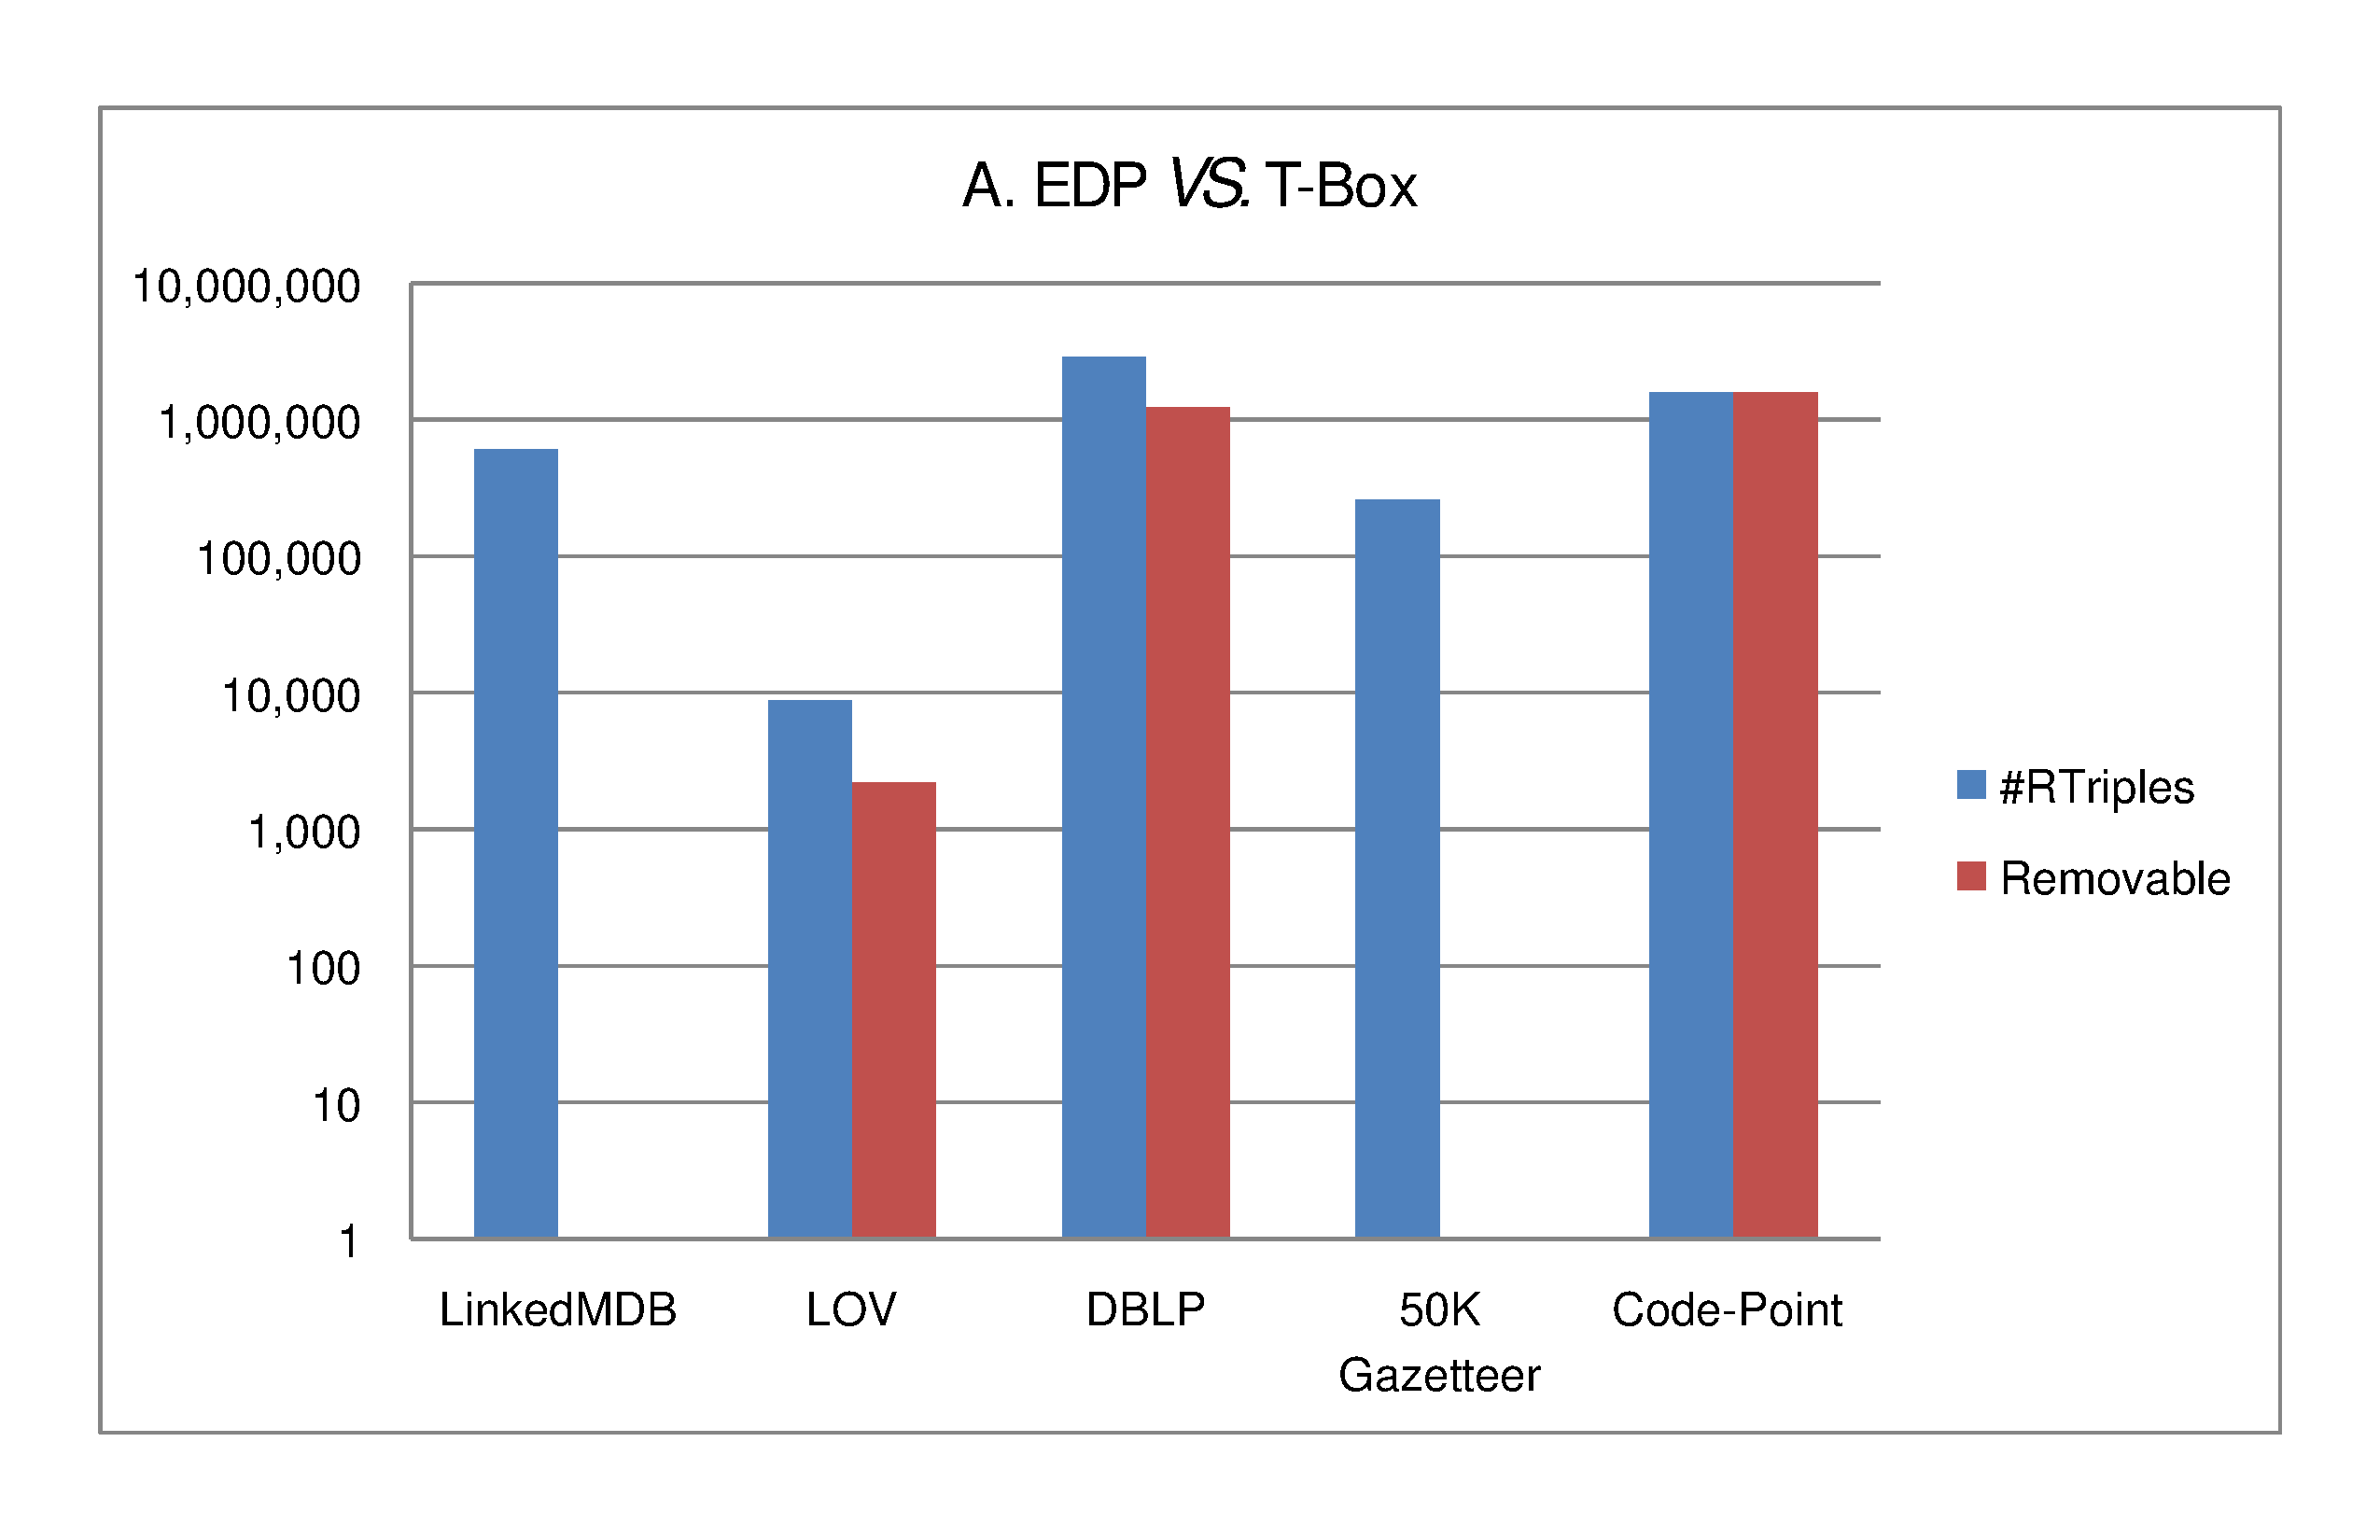
\includegraphics[scale=0.135, trim=0cm 0cm 0cm 2cm]{Figures/cmp_removable.pdf}   }   
    \hspace{2px}
 \mbox{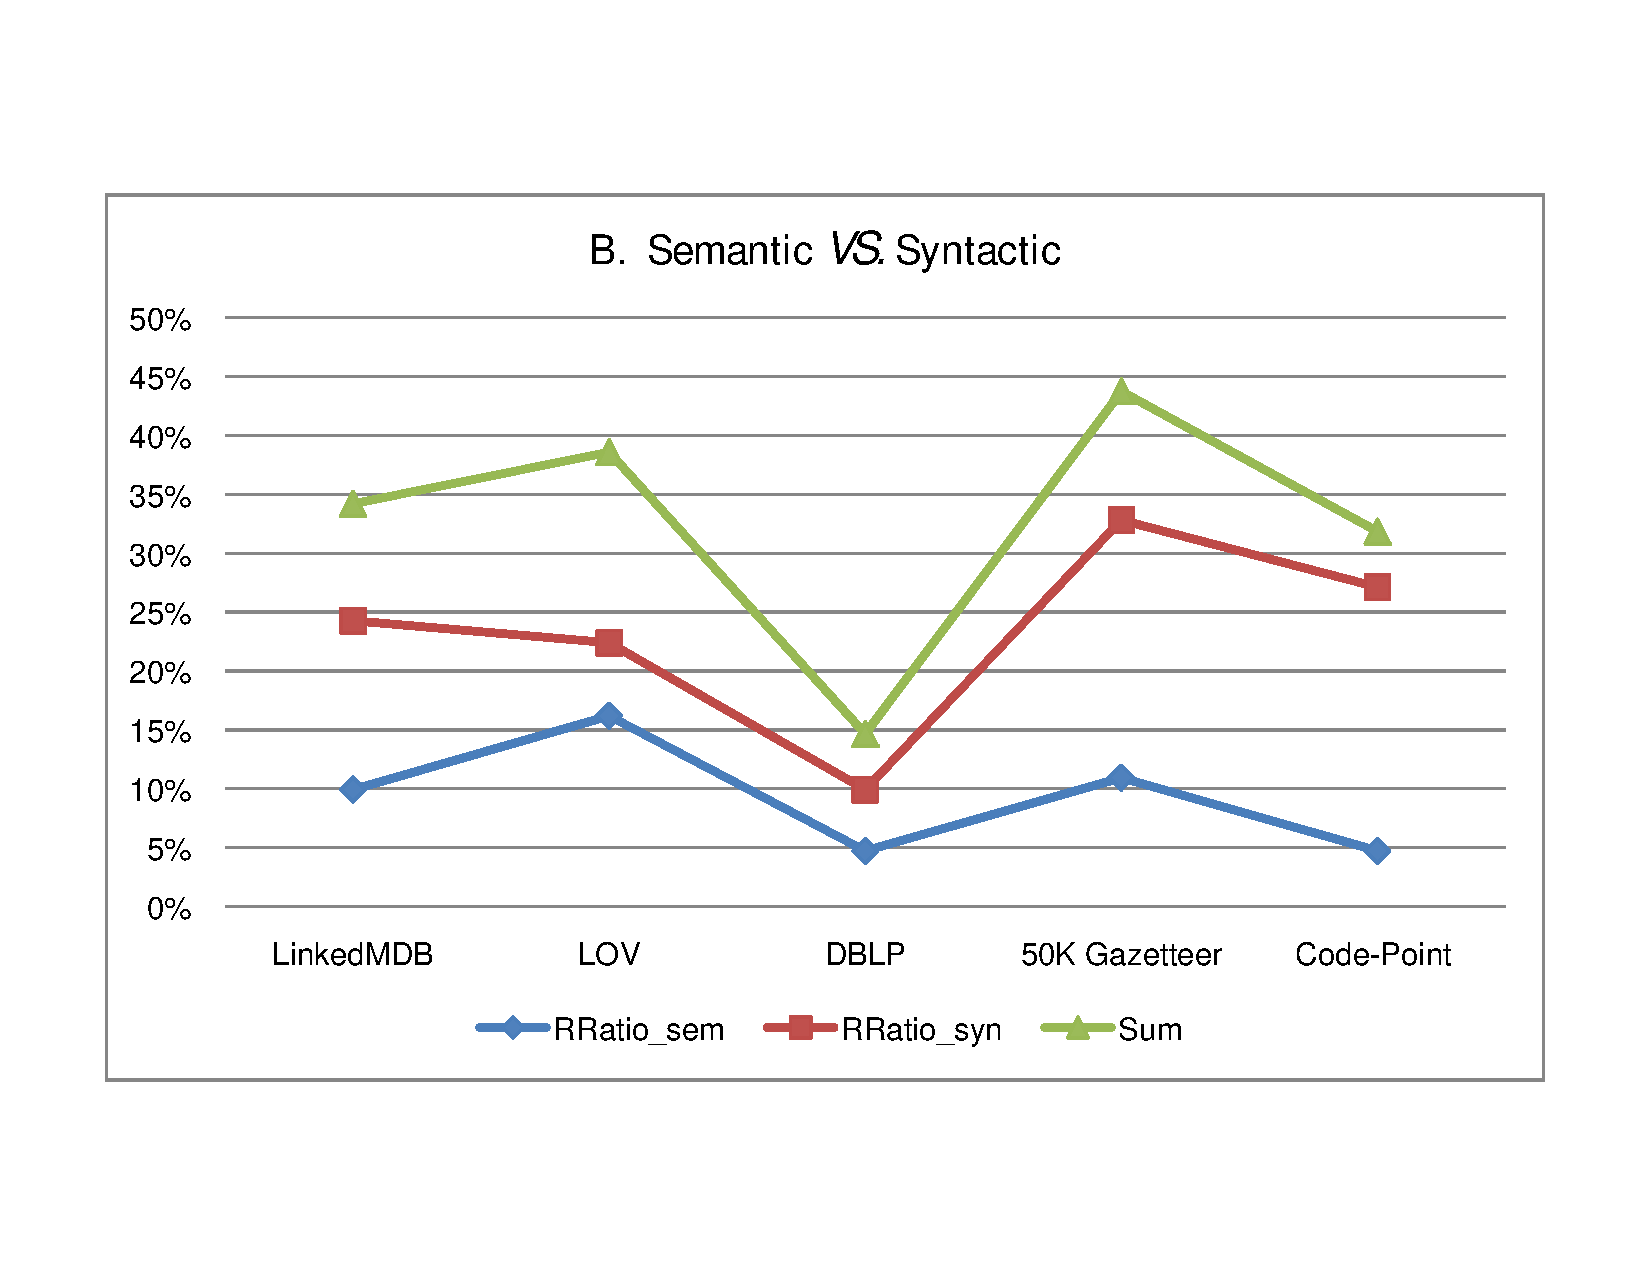
\includegraphics[scale=0.21, trim=0cm 2cm 0cm 2cm]{Figures/cmp_sem2syn.pdf}  }   
   \hspace{2px}
 \mbox{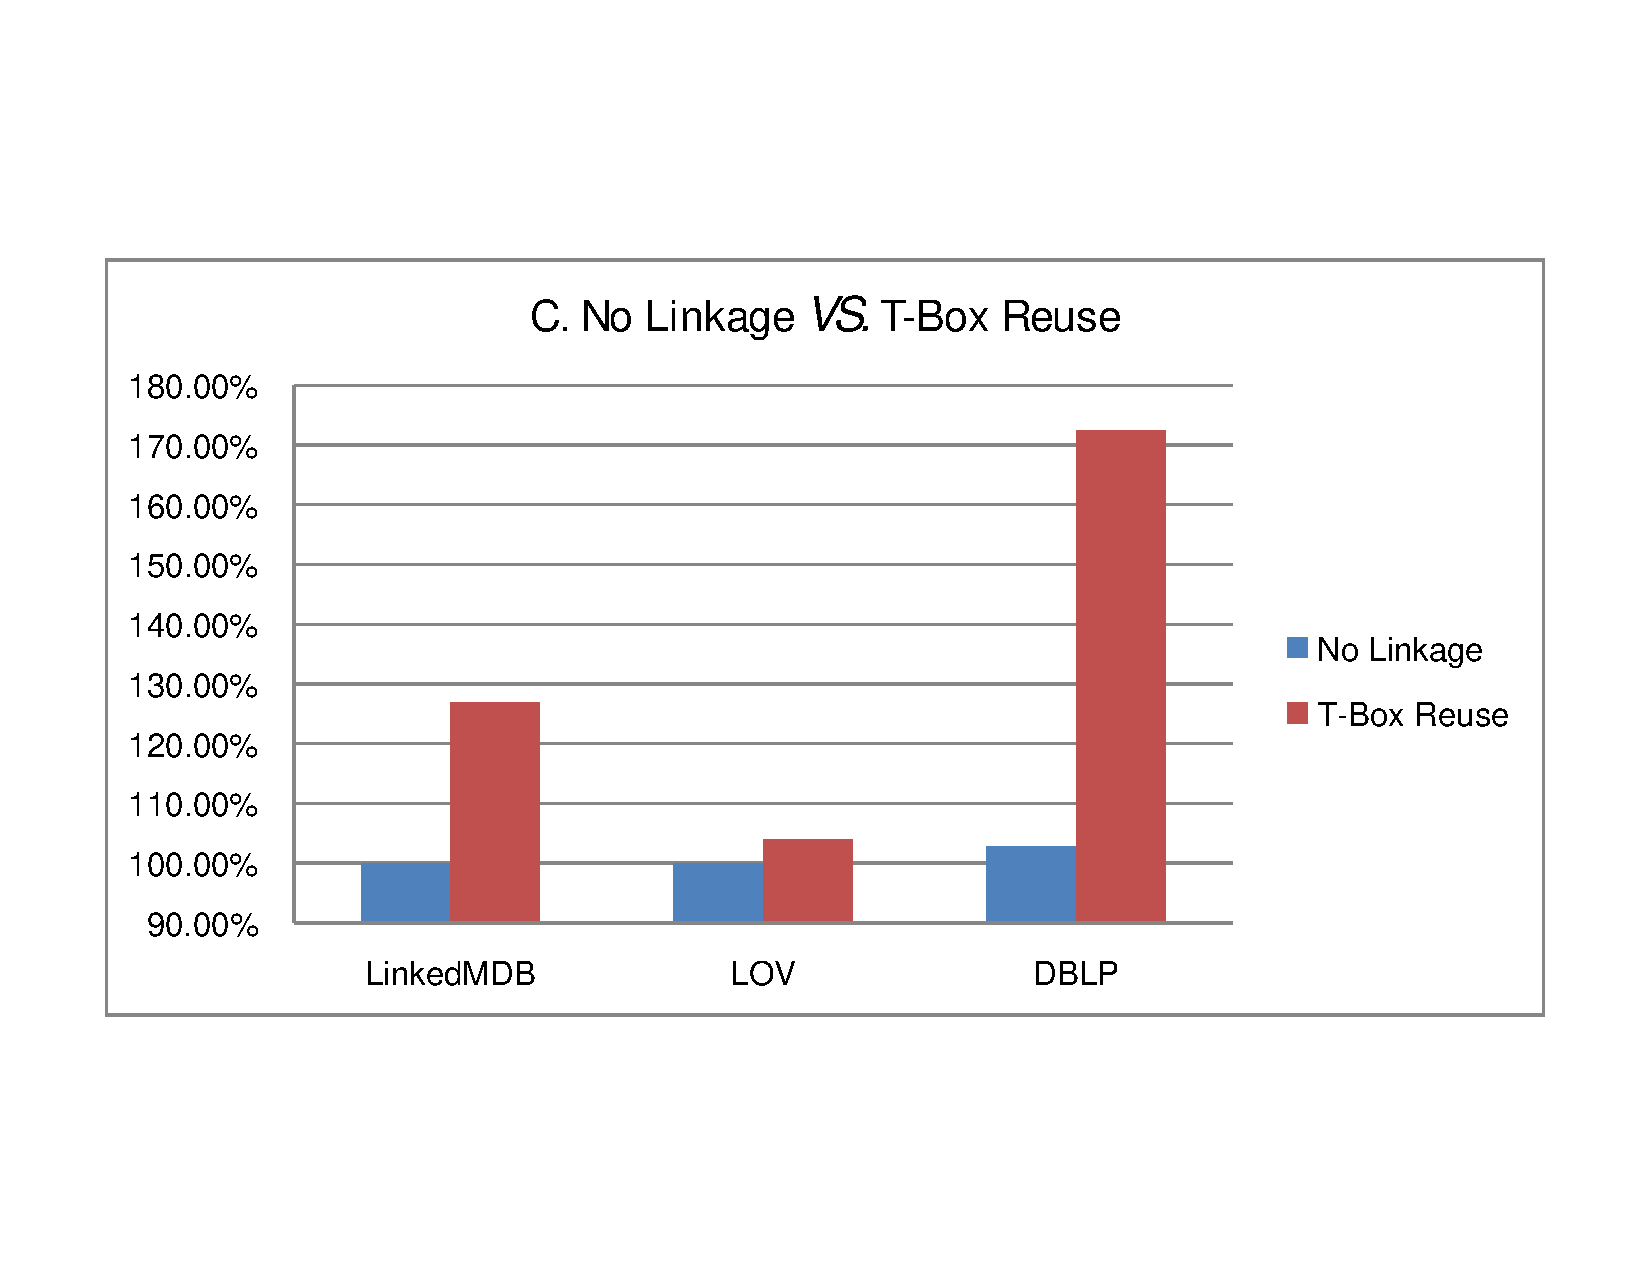
\includegraphics[scale=0.26, trim=0cm 6cm 0cm 2cm]{Figures/cmp_linked.pdf}  }   
\end{center}
\caption{Comparisons: \scriptsize A. {\it EDP VS. T-Box}; B. {\it Semantic VS. Syntactic}; C. {\it No Linkage VS. T-Box Reuse}. \normalsize}
\label{fig:cmp}
\end{figure*}

The top-right figure illustrates the comparison of semantic redundancy and syntactic redundancy. In all cases, the semantic one is less. The Sum of the two gives an idea about the overall data redundancies in these datasets. In 4 out of 5 datasets, the redundancy is more than 30\%. The largest one is in {\it 50K Gazetteer}, which has 44\% redundant data, and {\it DBLP} is least redundant dataset with about 15\% redundancy.

The bottom figure in Fig.~\ref{fig:cmp} shows the differences in the size of A-Box serialisation before and after T-Box reuse. In the figure, the size of serialisation is illustrated using the percentage: $Percentage=\frac{|\text{A-Box Materialisation}|}{|\text{Original A-Box}|}$. In all cases, the materialisations are increased by {\it T-Box Reuse}. Notably, there are more than 26\% increment for {\it LinkedMDB} and nearly 70\% for DBLP. 
\section{Conclusion}
\label{sec:conclusion}
In this paper, we introduced a systematic approach for analysing Linked Data redundancy. The most straightforward conclusion is that data redundancies in Linked Datasets are not only huge but also diverse. This leads to our main conclusion: {\it redundancy-aware techniques are demanded for both data consumption and data publishing}. The conclusion is broken down to several suggestions as follows.

\begin{itemize}
	\item {\bf For Data Compression} The compression tools or techniques should be aware that different types of redundancies exist. Different redundancies might need different techniques. Moreover, the knowledge of redundancy distribution is critical for tools which want to make a trade-off between efficiency and compression ratio.
	\item {\bf For Data Access} As shown in the results (cf. Table~\ref{tab:data}), data entities are described via different data patterns (EDPs). In most cases, the data distribution among EDPs is skewed, i.e. a small number of EDPs have a large number of data instances. For efficient data access purpose, the knowledge of such distribution and how to make use of it are critical.
	\item {\bf For OBDA and reasoning} It is obvious that A-Box redundancy can be utilised to avoid unnecessary rewritings. Moving a step forward from using rules equivalent to T-Box axiom to more general rule systems can improve the effectiveness of existing approaches significantly. 
	\item {\bf For Data Publisher} Being encouraged to link their data to other datasets, the publisher should be aware of the consequences of such linking in terms of bringing in $removable$ and $derivable$ triples. We have shown that a very small number of reuses can lead to a very large number of $derivable$. Publishers should be alarmed before creating links, and tools are needed to estimate such consequences and prompt them to the publisher.
	
\end{itemize}
%Data redundancy are huge: demands for compression techniques or compact representations
%
%Vocabulary linkage might lead to huge number of derivable triples
%Materialisation is not always an efficient way
%
%Redundancy aware techniques are demanded
%- how to make use of GP rules for consuming tasks
%- know categorisation of redundancy i.e., better indexing, compression
%- know which part is redundant, how to generate 
%
%Techniques:
%- generalised rule system 
%- inter-structural technique

\bibliographystyle{abbrv}
\bibliography{cold}
\end{document}


